\documentclass[border=4pt]{standalone}
\usepackage[compat=1.1.0]{tikz-feynman}
\tikzfeynmanset{every vertex={dot}}
\begin{document}
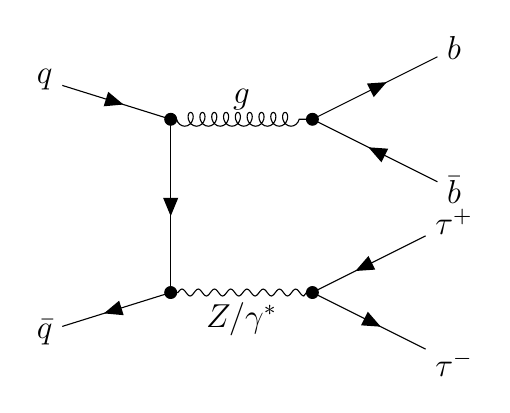
\begin{tikzpicture}[font=\large]
\begin{feynman}
\vertex (q) at (0, 1.6) {\(q\)};
\vertex (qb) at (0,-1.6) {\(\bar{q}\)};
\vertex [dot] (v1) at (1.6, 1.1) {};
\vertex [dot] (v2) at (1.6,-1.1) {};
\vertex [dot] (vz) at (3.4,-1.1) {};
\vertex (tp) at (5.2,-0.2) {\(\tau^{+}\)};
\vertex (tm) at (5.2,-2.0) {\(\tau^{-}\)};
\vertex [dot] (vg) at (3.4, 1.1) {};
\vertex (b) at (5.2, 2.0) {\(b\)};
\vertex (bb) at (5.2, 0.2) {\(\bar{b}\)};
\diagram*{
 (q) -- [fermion] (v1) -- [fermion] (v2) -- [fermion] (qb),
 (v1) -- [gluon, edge label=\(g\)] (vg),
 (vg) -- [fermion] (b),
 (bb) -- [fermion] (vg),
 (v2) -- [boson, edge label'=\(Z/\gamma^{*}\)] (vz),
 (vz) -- [anti fermion] (tp),
 (vz) -- [fermion] (tm),
};
\end{feynman}
\end{tikzpicture}
\end{document}
